\chapter{Results}

This chapter lists the temporary results from the experiments and thoughts on what it meant for the model, as well as the final results. All the experiments have been done on the same machine with: 11th Gen Intel(R) Core(TM) i7-11700K 3.60GHz 8-core CPU, 16 GB RAM and NVIDIA RTX 3080Ti graphics card.

\section{Progress}

In this section we will go throught the whole proccess step by step, from first iterations of the very simple model to more fine tuned models and other methods that were tested.

\subsection{Simple line graph model}

First step was to try the simplest model with most of the hyperparameters set to default and train it on a smaller scale. First model had 2 layers and 64 neurons each. Initially due to majority of nodes being not included in the matching, the model learned to set all nodes to be dropped and still get a rather high accuracy score. This was resolved by adding class weights as a training parameter. Class weights tell the model how important each class is. By assigning the nodes that go into matching a value of 0.9 and the ones that do not 0.1. The problem seemed to be resolved.
 
Trained on a 1000 MNIST graphs model resulted on average with 55\% of optimal weight possible. This was an expected result considering the limitation, but it at least showed that model is gaining some knowledge compared to untrained model as well as a solution that randomly picks edges, where both resulted in 50-51\% of optimal. 

A model that barely beats random solution is not very usefull. Poor performance for now is mainly to the very limited training, but before adding more data and prolonging training, we can experiments with the parameters of the network to see is they make any impact.

\subsection{Model improvements and data augmentation}

It would make sense to start with the depth and with of the network. After trying to add up to 6 layers in general it showed more than 3 layers did not have any significant effect. Note: layers tell how many generations of neighbors is used for representation of a node. Increasing breadth did help, but impact got smaller as the breadth got wider. It would also impact time consumptions so it was decided to have the model with 2 layers and 640 nodes at each layer (except input/output layers). Results were, however still rather low at  58\%.

Next step was to adjust optimizer parameters: learning rate and weight decay. 

Too high learing rates resulted in too unstable loss function, too low learning rate did not give enough progress and made training proccess too slow. Value of 0.001 worked well as middle ground

5. Weight decay

6. Trying skip connections, but not noticing any effect.

7. Augmenting node features. Trying each additional feature separately to see it they have any benefits by themselves, then adding them one by one. Finally using all at once since they can mostly be calculated simultaneously and all have at elast some positive effect:

\begin{figure}[H]
    \centering
    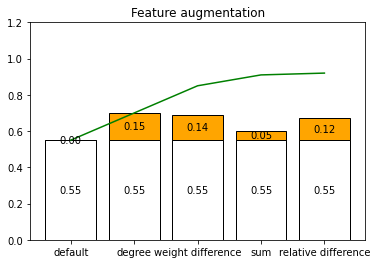
\includegraphics[scale=1.0]{figures/FeatureAugmentationLine}
    \caption{MNIST trained model. Average performance on 100 MNIST graphs}
    \label{Feature Augmentation Effect}
\end{figure}


With results starting to move closer to reasonable, now larger training set could be used. Unfortunately line graph transformation on a dense graph turned out to expode in size and take to much time to proccess. Therefore another architecture was considered. Trying edge classification. With same hyperparameters and repurposed node feature augmentation.
 
\section{Edge prediction model}

1. Edge classification is a little bit worse on average. In theory it can be due to line graph containing more structural information in it compared to original. 0.88\% of greedy

MNIST trained Model's performance on unseen MNIST graphs
\begin{figure}[H]
    \centering
    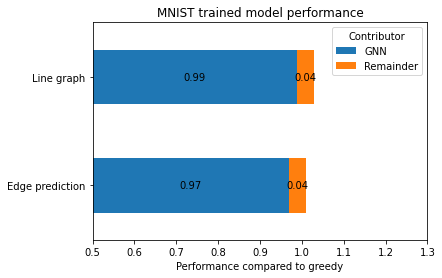
\includegraphics[scale=1.0]{figures/FinalPerformanceMNIST}
    \caption{MNIST performance comparison}
    \label{Model performance on MNIST}
\end{figure}

2. Trying to add a reduction rule and 2 additional features: 1st largest weight, 2nd largest weight for each node.

3. No noticable effect from neither reduction nor additional features.

4. Trying to train graph on the whole dataset of 55000 graphs:

RESULTS ON MNIST:

99\% of greedy, remainder <5%

RESULTS ON larger sage graphs:

sage 10: 0.86\% of greedy, remainder 0.53

\begin{figure}[H]
    \centering
    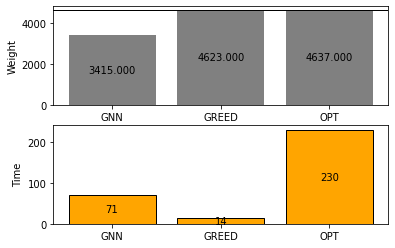
\includegraphics[scale=1.0]{figures/MNISTtrainSAGE10}
    \caption{MNIST trained model performance on sage10 graph}
    \label{model performance}
\end{figure}

5. Trying custom dataset of 1000+ graphs with varying sizes and structures, between 100 and 10000 nodes:

Results on MNIST: 

Results on larger sage graphs:

sage 10: 94\% of greedy, remainder =  0.54

\begin{figure}[H]
    \centering
    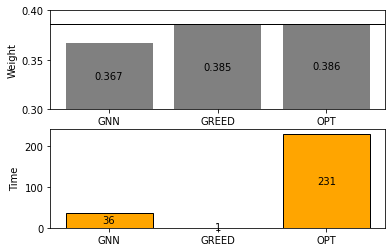
\includegraphics[scale=1.0]{figures/CUSTOMtrainSAGE10}
    \caption{CUSTOM trained model performance on sage10 graph}
    \label{model performance}
\end{figure}


6. Adjusting the threshold for the picking edges in to the solution and trying to remove edges below secondary threshold:

\begin{figure}[H]
    \centering
    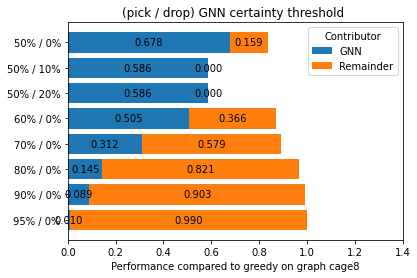
\includegraphics[scale=1.0]{figures/ThresholdDemo}
    \caption{Model performance on sage10 graph}
    \label{Model performance on sage10 graph}
\end{figure}


\section{Comparison of results}



\section{Final results}

Results of the best model (trained using CUSTOM dataset) on increasingly larger graphs:



\subsection{Weakness of greedy algorithm}

On average greedy seems to show realy good results, but in theory it is not hard to make a graph that abuses the greedy approach and results in poor performance. Example of a graph that \gls{gnn} model easily beats:

END
----------------------------------------------------------------------------------------------------------------------------------------
MISC NOTES IGNORE

Line graph vs normal vs normal with features (compared to standard greedy)

MNIST:
0.92 vs  0.77 vs  0.88 
Normal greedy remainder
LOW vs LOW vs LOW 

GOOD CASE data/Pajek/GD98b/GD98b.mtx:
1.43 vs  0.00 vs 1.00
Normal greedy remainder
LOW vs LOW vs LOW

MNIST 
----------------
GNN AVG Time =  0.1821751117706299
GREED AVG Time =  0.002601337432861328
GNN AVG Weight =  17.13489990234375
GREED AVG Weight =  17.2469970703125
remainder =  0.0440
----------------

trained on mix MIX


MNIST with reduction
----------------
GNN AVG Time =  0.2019108772277832
GREED AVG Time =  0.0028308868408203126
GNN AVG Weight =  17.117236328125
GREED AVG Weight =  16.9795166015625
weightResDif =  0.0355
----------------

trained on mix MIX

cage10 
--------------------------------------------
with reduction trained on MNIST

TIME
Opt AVG Time =  226.44823741912842
GNN AVG Time =  33.7434720993042
GREED AVG Time =  0.719895601272583
----------------
WEIGHT
Opt AVG Weight =  169.5332794189453
GNN AVG Weight =  123.09953308105469
GREED AVG Weight =  169.0205456027761
----------
weightResDif =  0.32484549283981323
-----------
END

TIME
Opt AVG Time =  238.8848557472229
GNN AVG Time =  35.6191520690918
GREED AVG Time =  0.8406157493591309
----------------
WEIGHT
Opt AVG Weight =  0.3864327073097229
GNN AVG Weight =  0.3369670510292053
GREED AVG Weight =  0.38539551471512823
----------
weightResDif =  0.5323471426963806
-----------
END

cage10 
--------------------------------------------
without reduction trained on MNIST

TIME
Opt AVG Time =  229.30790853500366
GNN AVG Time =  62.8546507358551
GREED AVG Time =  1.4378819465637207
----------------
WEIGHT
Opt AVG Weight =  169.5332794189453
GNN AVG Weight =  90.18408966064453
GREED AVG Weight =  169.06105741672218
----------
weightResDif =  0.5952541828155518
-----------
END

TIME
Opt AVG Time =  228.7730164527893
GNN AVG Time =  54.679471492767334
GREED AVG Time =  1.3367598056793213
----------------
WEIGHT
Opt AVG Weight =  0.3864327073097229
GNN AVG Weight =  0.2927633821964264
GREED AVG Weight =  0.38536409468088095
----------
weightResDif =  0.8586757183074951
-----------
END

cage10 
--------------------------------------------
with reduction, trained on MIX

TIME
Opt AVG Time =  226.55958795547485
GNN AVG Time =  38.985610246658325
GREED AVG Time =  0.7930364608764648
----------------
WEIGHT
Opt AVG Weight =  169.5332794189453
GNN AVG Weight =  133.77395629882812
GREED AVG Weight =  169.0205456027761
----------
weightResDif =  0.38094136118888855
-----------
END

TIME
Opt AVG Time =  230.7519097328186
GNN AVG Time =  36.04787516593933
GREED AVG Time =  0.709648847579956
----------------
WEIGHT
Opt AVG Weight =  0.3864327073097229
GNN AVG Weight =  0.36708855628967285
GREED AVG Weight =  0.38539551471512823
----------
weightResDif =  0.5425851345062256
-----------
END

cage10 
--------------------------------------------
without reduction, trained on MIX

TIME
Opt AVG Time =  237.57963299751282
GNN AVG Time =  63.44921660423279
GREED AVG Time =  1.4237451553344727
----------------
WEIGHT
Opt AVG Weight =  169.5332794189453
GNN AVG Weight =  116.88045501708984
GREED AVG Weight =  169.06105741672218
----------
weightResDif =  0.7212029695510864
-----------
END

TIME
Opt AVG Time =  220.3951222896576
GNN AVG Time =  59.582497119903564
GREED AVG Time =  1.435647964477539
----------------
WEIGHT
Opt AVG Weight =  0.3864327073097229
GNN AVG Weight =  0.35216498374938965
GREED AVG Weight =  0.38536409468088095
----------
weightResDif =  0.837394654750824
-----------
END


----------------------------------------

cage11  

without reduction

TIME
Opt AVG Time =  1624.2668080329895
GNN AVG Time =  90.85399174690247
GREED AVG Time =  2.7126402854919434
----------------
WEIGHT
Opt AVG Weight =  793.24462890625
GNN AVG Weight =  595.8353271484375
GREED AVG Weight =  790.162699168548
----------
weightResDif =  0.39534446597099304
-----------
END


NOT line NN graph MNIST weights normalized vs MNIST weights ones vs MNIST weights 1-2 vs MNIST weights 1-5
0.88 vs 1.00  vs 0.83 vs 0.60

\section{Performance on unseen data}

\begin{center}
\begin{tabular}{||c c c||} 
 \hline
 Algorithm & Time & Weight \\ [0.5ex] 
 \hline\hline
 GNN & 1 & 6 \\ 
 \hline
 Greedy & 2 & 7 \\ [1ex] 
 \hline
\end{tabular}
\end{center}

How well the final model solves the matching problem